\documentclass[a4paper,12pt, twocolumn]{article}
\usepackage{graphicx}
\usepackage{float}
\usepackage{titling}
\usepackage{geometry}
 \geometry{
 a4paper,
 total={170mm,257mm},
 left=25mm,
 right = 25mm,
 top=20mm,
 }

\title{Is there correlation between temperatures in consecutive years in Florida?}
\author{Tianle Shao}
\date{\today}

\begin{document}

\maketitle

\section{Introduction}
This investigation makes use of temperature data from Key West (Florida, USA) over a period of 100 years from 1901 to 2000, to determine if the temperature of consecutive years are correlated with each other. The presence of such a correlation may have implications on the changing local climate, with an increasing trend possibly suggesting the impact of climate change on the Floridian climate, giving basis for further action to be taken on the policy level to combat such changes. Being an area containing unique ecosystems including the Florida Keys, it is integral that such an ecosystem is kept intact in the face of a changing climate.

\section{Methods}
The correlation between consecutive years' temperatures was calculated using the Pearson correlation coefficient. A permutation analysis with 10,000 random repeats was performed, where the Pearson correlation coefficient for these repeats were calculated and compared with the correlation coefficient of the temperature data.

\section{Results}
  \begin{figure}[ht]
    \centering
    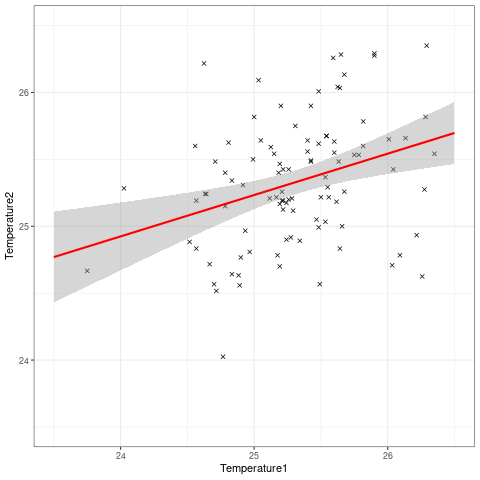
\includegraphics[width=0.5\textwidth]{../data/ats_plot.png}
    \caption{Temperature between consecutive years}
  \end{figure}
  
  \begin{figure}[h]
    \centering
    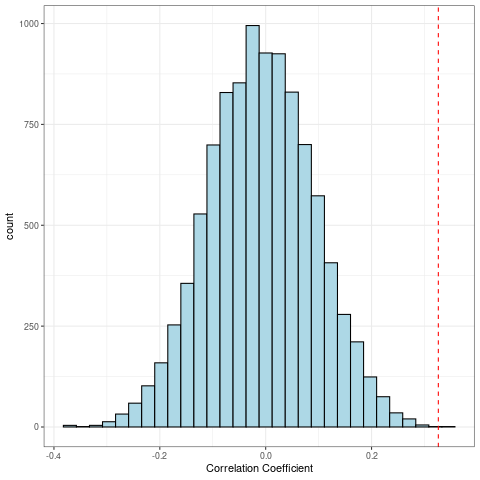
\includegraphics[width=0.5\textwidth]{../data/ats_random_plot.png}
    \caption{Statistical distribution and count of correlation coefficients.}
  \end{figure}
  \noindent The correlation coefficient was found to be 0.3261697, suggesting a weak, positive correlation between temperatures of consecutive years in Florida (Figure 1). Through $10,000$ random permutations, it can intuitively observe from the graph that the vast majority of the test correlation coefficients are distributed around 0 (Figure 2). The red dashed line in the graph represents the correlation coefficient from the initial test without random event sequencing (Figure 2). It is evident that almost all the test correlation coefficients are greater than the initial correlation coefficient. This also indicates that there is a correlation between the initial temperature and the time series. A majority of the 10,000 random permutations resulted in a correlation coefficient spread around 0. The red dashed line in the graph represents the correlation coefficient of the Florida temperature data, which is further from 0 than 99.93\% of random permutations, suggesting that the weak, positive correlation observed is significant. \\
  
\section{Discussion}
\noindent These results imply that the Florida Keys have been slightly increasing in temperature over 1901-2000, which could be due to temperature change on a local or global scale. This is importance to ecosystem stability, due to the effect of temperature on organism physiology and metabolism, as well as behaviours including reproduction and migration. Further studies will need to be done to confirm this trend, and its potential effect on organisms and ecosystems.

\end{document}
